%% The first command in your LaTeX source must be the \documentclass command.
%%
%% Options:
%% two-column: Two-column layout.
%% hf: enable header and footer.
\documentclass[
% twocolumn,
% hf,
]{ceurart}
\usepackage{amsmath,amssymb,longtable,hhline}
\usepackage{doi}
\def\doitext{DOI:}

%%
%% One can fix some overfills
\sloppy

%%
%% Minted listings support
%% Need pygment <http://pygments.org/> <http://pypi.python.org/pypi/Pygments>
% \usepackage{listings}
\usepackage{minted}
\setminted{fontsize=\footnotesize,mathescape}
\usepackage{hyperref}
\usepackage{multicol}

\hypersetup{
    bookmarks=true,         % show bookmarks bar?
    unicode=true,           % non-Latin characters in Acrobat’s bookmarks
    pdftoolbar=false,        % show Acrobat’s toolbar?
    pdfmenubar=false,        % show Acrobat’s menu?
    pdffitwindow=false,     % window fit to page when opened
    pdfstartview={FitH},    % fits the width of the page to the window
    pdftitle={},    % title
    pdfauthor={Evgeny Cherkashin},     % author
    pdfsubject={Technologies of Semantic WEB as an environment of application development and integration},   % subject of the document
    pdfnewwindow=true,      % links in new PDF window
    colorlinks=true,       % false: boxed links; true: colored links
    linkcolor=black,          % color of internal links (change box color with linkbordercolor)
    citecolor=black,        % color of links to bibliography
    filecolor=black,      % color of file links
    urlcolor=black           % color of external links
  }
\urlstyle{tt}
\usepackage{pifont}
\usepackage{xcolor}
\graphicspath{{pics/}}

\newcommand{\GB}[1]{\colorbox{green}{#1}}
\newcommand{\BB}[1]{\colorbox{blue}{#1}}
\newcommand{\RB}[1]{\colorbox{red}{#1}}


%% auto break lines
% \lstset{breaklines=true}

\newcommand{\ns}[1]{\textbf{\texttt{#1}}}

%%
%% end of the preamble, start of the body of the document source.
\begin{document}

%%
%% Rights management information.
%% CC-BY is default license.
\copyrightyear{2021}
\copyrightclause{Copyright for this paper by its authors.
  Use permitted under Creative Commons License Attribution 4.0
  International (CC BY 4.0).}

%%
%% This command is for the conference information
\conference{2nd International Workshop on Advanced Information and Computation Technologies and Systems, December 6--10, 2021, Irkutsk, Russia}

%%
%% The "title" command
\title{Distributed Environment for Auctioning Virtual Power System Resources}
%%
%% The "author" command and its associated commands are used to define
%% the authors and their affiliations.
\author[1,2]{Mikhail A. Chekan}[%
orcid=0000-0003-2428-2471,
email=eugeneai@icc.ru,
url=https://github.org/eugeneai,
]
\author[1,2]{Evgeny A. Cherkashin}[%
orcid=0000-0003-2428-2471,
email=eugeneai@icc.ru,
url=https://github.org/eugeneai,
]
\address[1]{Matrosov Institute for System Dynamics and Control Theory of Siberian Branch of Russian Academy of Sciences, 134 Lermontov St, Irkutsk, 664033, Russian Federation}

\address[2]{Institute for Mathematics and Information Technologies, Irkutsk State University, 20~Gagarina Bulv, Irkutsk, 664003, Russian Federation}


\begin{abstract}
  The paper discusses the development of an auction environment used as part of a ``smart grid'' simulator. Usage of the Haskell programming language, the Nix package manager, and a set of architectural solutions, such as the relative time windows and the SSH tunnel-based network architecture, made it possible to create a flexible and reliable system. This system was successfully applied both in distributed and in high-load local scenarios.
\end{abstract}

\begin{keywords}
  distributed systems \sep auctions
\end{keywords}

\maketitle

\section*{Introduction}
\label{sec:into}

The current trends in energy sector organizations in the developed countries (including Russia) pay special attention to the concept of ``smart energy.'' The environmental and economic situation forces them to optimize energy processes, switch to alternative sources, and introduce smart grids [1]. Information technologies play a special role here as implementers of a ``smart energy'' control. In this regard, the issue of training specialists with a comprehensive understanding of energy processes as being based on modern technologies is relevant. On the other hand, smart energy has not yet found good distribution at the household level in some countries. One of the effective methods for dealing with these issues is devising tools for specialized training of young specialist-engineers. The proposed game component plays an essential role in the educational effect, an energetic auction modeling tool as additional didactic material~[2].

The control synthesis is mainly based on the sequence of ``energy market players'' decisions. One of the possible ways of developing the capabilities is to organize the game based on a computer simulation of the operation of the power system. The particular product is the training stand ``Intelligent Energy Systems'' (denoted as \emph{powerstand})~[3], developed by Polyus-NT~Ltd. It allows a tutor to show the basics of planning and managing a real power supply network in a smart grid context. The product has been implemented and deployed in several quantoriums in Russia and used at major educational events, including the final stage of the track of the same name at the annual National Technological Olympiad (NTO). The product can be adapted to various kinds of customers, including industries.

The powerstand game session consists of stages. One of the stages is auctions for the ownership of objects of a playing ground district assembled by the participants of the power grid. The grid is subsequently simulated, accounting parameters of energy efficiency and profitability. Since the set of objects directly impacts the simulation result, it is crucial to carry out reliably and promptly this stage of work with the stand. The problem is the imperfection of the manual auction version when the hosts independently collect the participants' bids using material (paper) or digital media (messages in a messenger application). We proposed automating this stage and introducing it into the existing software packages to improve reliability. Power system modeling is an already essentially automated process. Reducing external dependencies through additional automation will increase the integrity of the software and hardware complex and increase the dynamics of the activities, as well as reduce the requirements for operator qualification requirements, which is especially important when deploying the stand as an educational tool at various sites where the direct presence of administrators is not expected.

The first version of software was successfully developed and implemented as a powerstand module~[4]. However, as the popularity of virtual formats of educational and competitive events grows, it becomes necessary to implement an extension of the module for supporting the distributed environment of virtual auctions when participants work at stands located in different geographically distant points. The result of designing and implementing such an environment is presented in the research.

This research and development aim to construct an efficient (in terms of the reaction speed and maintainability) distributed environment to provide game activities enabling students to conduct and participate in auctions as a part of a smart energy training stand.

The theoretical base of distributed software systems has a significant degree of development. Some works consider its aspects in detail [5]. In particular, centralized architectures and their variations (client-server, three-tier, n-tier) are well studied. Therefore, in terms of architecture, modern works [6] pay much attention to distributed decentralized (peer-to-peer) architectures, in particular, based on blockchain [7]. Since the auction environment is designed to be implemented in existing systems with a closed architecture, and the implementation of the game logic requires an arbiter in the form of a central node, a decentralized approach in the current state of work is considered suboptimal. It is also due to the complexity of implementation and support. However, as part of the hypothesis for further research, the use of a decentralized architecture is considered, including implementing the free organization of gaming sessions.

Building a network architecture with the expectation of implementation in consumer products involves following the standards for building computer networks that have been formed over the past half-century, including the OSI model and the protocol group of the transport and session layers of this model [8]. These standards have been tested by time and practice, so the task of developing and designing new solutions belongs to the application and session levels, while solutions at the session level and below are most often the \emph{de facto} standard, and working with them comes down to choosing options.

In addition to technical standards, there are fundamental requirements for a distributed system, mentioned in the book by W. Jia and W. Zhou. Among these requirements, it is worth highlighting competitiveness (system nodes operate in parallel), openness (the ability to freely use and expand), fault tolerance (recoverability after errors and failures), and security (in particular, the suppression of external interference in the system). The proposed solutions must meet these requirements and be simple to implement. In particular, if we consider the software package as a combination of software modules and the execution environment, the developer has at his disposal system utilities that have already been implemented and debugged to a sufficient extent to delegate part of the functionality to them.

Jia and Zhou also mention replication to provide fault tolerance [5, p. 240]. In addition, replication solves two more problems - increasing the availability of the service (if one node fails, the functionality supports the other) and improving performance (reducing response time by distributing the data flow across different servers). Although these provisions are described mainly for decentralized systems, replication in a centralized architecture (if we consider working with data separately) also allows them to be achieved.

Software solutions for implementing distributed architectures are often reduced to embedded libraries for network interaction and message passing. It is worth highlighting libraries for implementing remote procedure call (RPC), particularly gRPC [9], a full-fledged cross-platform solution for distributed computing. However, the most common solutions related to remote message passing require utilization of other libraries that pull additional dependencies. It makes sense to write code for network functionality optimized for specific conditions and requirements depending on the task.

There is no consensus on the issue of organizing a network infrastructure, namely, connecting services, and most typically, services interact through open channels using TCP and UDP protocols. This option provides sufficient throughput and, in the case of TCP, consistent two-way communication but imposes security and network infrastructure requirements. Problems regarding network infrastructure most frequently lie in the configuration of routing and access ports, and security issues are addressed through various add-ons related to encryption and authorization mechanisms. The most popular access control protocol at present is OAuth [10]. There are ready-made solutions [11] that implement interaction using this protocol. To protect applications from denial of service attacks, balancers are used, \emph{e.g.}, NGINX [12].

There are scenarios where it is necessary to block access to the application from the external network to everyone except trusted nodes, namely, in corporate systems. To implement such scenarios, VPN tunneling, access via a terminal connection (for example, VNC), and web interface publishing via HTTPS [13] are often used, and the latter method prevails by author's opinion. VPN tunneling is considered the most popular and common method of creating a closed channel between nodes. However, its use is associated with some risks and requires proper configuration. The same applies to a web application. The terminal connection is used mainly for organizing user interaction with the desktop (VNC is used for this). At the same time, the SSH protocol, in addition to its primary functionality - remote interaction with the user environment - provides tunneling of TCP connections over an encrypted channel [14]. To organize a simple SSH tunnel, two nodes are enough, where an SSH server is installed on one, and an SSH client is installed on the second, launched with a specific set of arguments. Both components come standard with many Linux distributions [15]. The further configuration depends on security and infrastructure requirements.


\section{User experience analysis}
\label{sec:user-exp}

The auction, as mentioned above, the module has become a prototype of the distributed environment. Being a part of a powerstand software, the module is used in educational institutions, engineering competitions, and intensive programs. During the powerstand operation and administration and personal observation of auction system operation, a significant amount of user experience was accumulated, based on decisions made regarding developing new versions of software products and creating unique technical solutions. This experience has become the primary source of expertise in forming requirements for a new interpretation of the auction system in distributed scenarios. Three events made the dominant contribution to the expertise. This section will describe them and briefly analyze the user experience.

The first auction module application was at the finals of the “Intelligent Energy Systems” profile of the 2018 NTI Olympiad [16] at the Sirius Educational Center in Sochi. Even though the module was still in the prototype stage and the game model was more straightforward than manual conduct, the auction automation significantly improved the quality of the game session. Bets were sent directly from the teams’ workplaces, and the round result was determined automatically. That increased the game dynamics, eliminated organizational costs, and brought a positive experience to the process.

The educational intensive program ``Island 10-21'' in the same year from July 10 to July 21 at the Far Eastern Federal University (Russkiy Island) [17]. A modified version of the auction module was used as a part of a stand at a ``smart energy'' educational laboratory. The game model was brought to the current one, the same as in the manual auction. The administrator and observer interfaces were added. The developer was personally present at the event, administering the stand and observing the laboratory conduction. Due to the higher speed of the game and rapid UI feedback, the automatic auctions' usage makes the object distribution fast and dynamic. Playing at the auction evoked positive emotions among the laboratory participants. Displaying auction results through a projector added spectacle to the process and allowed outside observers to track and analyze auction results in real-time. The administrator's interface turned out to be necessary only for the game session starts and restarts, as well as occasional pauses to describe the game situation.

Nevertheless, it turned out to be very useful in terms of information content, as it displayed bids for the current lot (the participants themselves see only the fact of the decision made by the opponent). It allowed the organizers of the educational program to track the participants' behavior and make decisions on further work within the laboratory.

From March 13 to March 17, 2019, the IPS profile finals of the NTI Olympiad took place. It was the first profile final in a distributed format and the first experience of distributed games on the powerstand. The competition was at two venues: the MEPhI Nuclear Research University (Moscow) and the Scientific Library of Irkutsk State University. Most of the stand software was done from scratch for the new game and architectural model. The auction module remained intact, except for a slight modification of the game model and adaptation of the interface for eight players. Thus, the user interface was interacting with the server part of the auction module hosted on the cloud server.

The rules of the event included practice games both in distributed and local formats. Local format implied the core services (incl. the auction module) to be placed in the stand instead of a cloud server. A service manager was implemented to set up and monitor applications based on a configuration file to perform mode switching. In practice, the service manager became a source of hard-to-diagnose bugs but still managed to complete the task.

The result of the final was ambiguous due to technical problems associated with an unstable communication channel on the Irkutsk site, which also held the finals of two more profiles. The protocols of the stand software modules were not adapted to low bandwidth networks, which caused noticeable delays for 5-6 s on average. They were noticeable, disrupted the automatic auction dynamics, and created unequal conditions between sites. Latency was negatively impacted by a query time limit issue in the web framework used. Backend requests took a lot of time in addition to JSON state deserialization (due to a complex structure and more than 100 kilobytes size). Thus, the delays increased to those values ​​at which participation in the auction became difficult. There was also a desynchronization: the round countdown was based on the UNIX timestamp created on the cloud server, while the clock on the terminal could differ from the server clock by more than a few seconds, which, together with the delay, created a situation when the bet was sent but came to the server too late. Despite the current situation, organizers managed to conduct training and final games correctly. Nevertheless, after this event, we decided to review the network architecture organization and the protocol of all stand modules to obtain more stable operation in the conditions of low-quality or slow communication channels. Within this direction, the idea of ​​this work arose.

During observation and experiments related to the auctions module, it was found that a 1-2 second delay in switching the state of the auction does not disrupt the dynamics of the auction process. JSON packets up to 100 kilobytes in size are processed by the browser within a second, which fits within the allowable time with a good communication channel.


\section{Requirements}
\label{sec:reqs}


The powerstand specificity determined the game model, namely its succession to the previous version. Also, the technical component of the stand determined the basic architecture of the environment, consisting of three levels:
\begin{itemize}
\item the cloud level, which implements the logical core of the stand (game session control, game logic);
\item  the stand (relay) level, which coordinates data transfer between the cloud and terminals;
\item  the terminal (interface) level, which implements the user’s interaction and transfers one's actions to the upper levels.
\end{itemize}

The terminal and stand levels exist close to each other as a part of a powerstand. Client stations implement the terminal level and are connected to the controlling unit with the powerstand server inside. Clients and servers are connected via a wired LAN, and the router used for it provides bandwidth up to 1 Gb/s. It provides a high-speed and low response time for communication between terminals and relays. At the same time, data can be transmitted openly, which creates a potential vulnerability in the normal gameplay: a third-party client can intercept the data stream and disrupt the game, ranging from a gameplay disbalance up to system failures. It implies network security and also enables us to implement static module authorization. For example, the configuration of terminals is known in advance, and it can be set strictly statically in one or another module of the system.

In the base scenario (such as holding events using power stands), the system architecture assumes the presence of several such physical stands located at geographically different points and connected to a cloud server. This arrangement implies heterogeneity of network channels and, as a result, the problem of synchronization of transmitted data and control actions. From this follows the requirement for leveling network delays. The helping fact is that the auction gameplay consists of rounds that do not require strict synchronization, but only relative simultaneity (difference within 1-2 seconds is allowed) and equality of a countdown on all stands. It is based on centralized game logic: the cloud level sets the game’s pace, accepts actions from players and physical objects from all stands, processes them, and sends out updated data.

Recalling the third-party interference problem, the data transfer and user actions are required to be minimally subject to outside interference with the relative ease of authorization and connection of modules to each other.

Thus, the resulting network is heterogeneous: there is a high-speed intra-stand network level and an inter-stand layer associated with data transmission through the core. However, there may be a hardware or software problem at both levels, for example, network channel instability or involuntary disconnection of terminals. The solution would be to implement a system that would continue a game session on a module failure and which modules can quickly recover from such a failure.

Finally, the requirement for architecture is its flexibility. So, stand usage scenarios include the possibility of disconnecting the stand from the cloud server for local gaming sessions (standalone mode). In this case, the cloud level is situated at the same physical place as the relay level. It is expected that the stand reconfiguration to a single-mode will require minimal effort and will have minimal impact on the source code of game services.

Based on the experience described above, and the sources studied, the requirements for a distributed environment for conducting virtual auctions have been formed: the implementation of a stable dynamic architecture with the following properties:
\begin{itemize}
\item minimizing the risks of external interference while maintaining the simplicity of connecting and authorizing modules (considering their known configuration);
\item leveling network delays while maintaining the relative synchronization of the game session and the equality of the duration of cycles;
\item system stability preservation in case of a child module failure and fast module recovery in such a case.
\end{itemize}

Game model (перевести картинку)

The construction and justification of the game model are based on the statements of the auction theory, which studies auctions as microeconomic models using game theory. Its accessible and popular presentation was made by A. Filatov and A. Savateev [18]. One frequently mentioned statement is the revenue equivalence theorem, proven by R. Myerson [24]. According to this theorem, the average revenue of the seller and the expected payoffs of the participants do not depend on the model and rules used, provided that three conditions are met:
\begin{enumerate}
\item ``No entry ticket'': the participant with no lot evaluation pays nothing.
\item The lot is always given to the participant with the highest bid.
\item Bid evaluations of auction participants are distributed independently and equally (that is, symmetric equilibrium is presented).
\end{enumerate}

All these statements are true in the context of the chosen applied task, from which we can conclude that it is possible to freely choose the auction format (as well as their combinations) for use in the game model. Thus, the first-price sealed-bid auction is used as a game model. The use of a sealed-bid format is caused by its resistance to short time delays, in contrast to the open dynamic formats such as English and Dutch auctions, where the order of bids is important. It ensures the highest possible equality of conditions among bidders in distributed scenarios.

Lots are put up for auction, which in the applied task are game objects, buildings with an individual address. Participants write bids for the declared lot and send them sealed (without revealing them to competitors) to the host (a person or an automated system).
The bid value has a predetermined limit range, which is individual for each lot (in the applied task, it depends on the object type). Such a restriction is set to form a sensible economic situation. The bottom limit comes from considering that all objects have value, and the upper limit protects participants from excessive losses in an upward auction and excessive profits in a downward auction.
In addition to sending the bid, the participant can refuse to bid on the lot (namely, pass it). Passing does not incur sanctions and penalties to the participant (principle of ``no entry ticket'').

The bid time is limited by a countdown timer, after which the bids are compared. They are sorted in ascending or descending order depending on the type of lot: for consumption objects, rates are tariffs per power unit and are compared downwards; for generation objects, the rates are the rent per game tick and are compared upwards. If the winner is unambiguous, the lot is closed and assigned. If no single bid has been made on the lot, it is declared unplaced and does not participate in the further game at the stand.

The situation is possible when several participants’ evaluation is almost the same, but the probability of an exact match of their rates is insignificant. Therefore, ``catching up'' bids are used for a more competitive distribution of lots. If some bids differ from the leading one by less than 0.5 money units, another round is held for the same lot with the leader and owners of ``catching up'' bids.

If one of the participants has bid a limit price (for example, the minimum value in a downwards auction), then the ``catch-up'' bid mechanic does not work, and the lot is assigned to this participant. If two or more participants set the limit bid, a new round is announced on the all-pay principle. There, bids are fixed amounts that bidders are willing to pay to get the lot at the marginal price. However, regardless of the outcome, the bet sent by the participant is debited from his account as a penalty. In the main game, the total value of the penalty for all-pay is deducted from the initial score.

Given the conditions for revenue equivalence, we can consider an all-pay auction to be equivalent to a sealed-bid first-price auction in determining value. By bidding on the limit value, the participants set the personal value of the object, sacrificing its objective value (economic effect). To resolve the disputable situation, the personal value is determined again by bidding on the amount the participant is willing to give to own the object. Since the increase in this value negatively affects the final result of the participants, it was decided not to apply the ``catch-up'' bets rule in all-pay, holding a second round only if the leading bets completely match.

After the first auction pass, when the objects are pre-assigned, participants can refuse a certain number of their lots, putting them on the second pass of the auction, along with those that were unplaced on the first. In case of refusal of a lot, the participant loses the right to compete for this lot. The value of the refused lots is then determined anew (that is, the bid range is reset to the original one).

At the end of the auction, the results tally is generated to represent information about the ownership of the objects, the bids set on them, and the submitted all-pay bids.

According to the game model described above, a state diagram is drawn, shown in Figure~\ref{fig:1}.


\begin{figure}
  \centering
  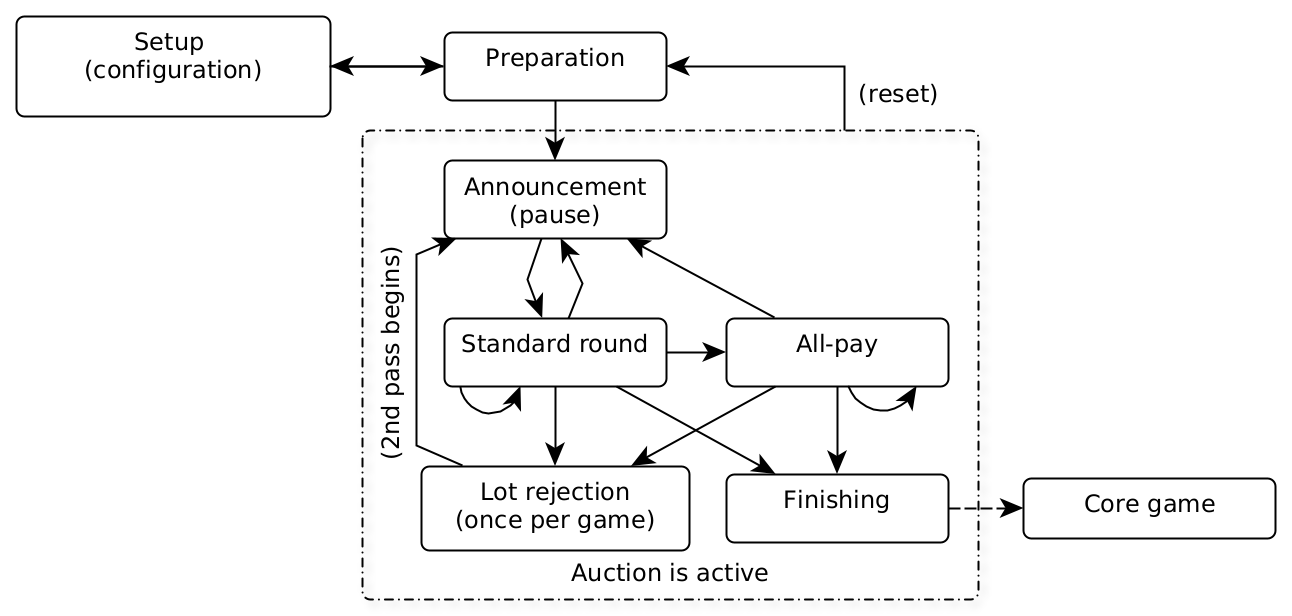
\includegraphics[width=0.7\linewidth]{pics/statechart.png}
  \caption{Auction state model}
  \label{fig:1}
\end{figure}

This model allows simultaneous independent draw of several lots. This further increases the dynamics and cognitive complexity of the auction, forcing participants to more carefully coordinate their decisions about the value of the lots to keep pace with the pace of the auction.

The described model is abstract enough and contains almost no binds to the stand domain. Therefore, the model enables solving other tasks related to the distribution of virtual resources. It is also possible to change the model implementation, if necessary, i.e., add additional rules.

\section{Implementation architecture}
\label{sec:impl-arch}

A three-level hierarchical architecture is implemented as a result of the analysis of existing developments in networks and distributed systems. For convenience, we also divide it into three layers: system (operating system tools), software (implementation of server and client programs), and transport (protocols and data transfer principles).

We note the need for stable and consistent two-way data transmission in the transport layer. The TCP protocol successfully performs it, so it became the transport core. Typed messages are sent over the established connection. Although it is possible to re-implement the stream-based protocol with length control, it was decided to use the WebSocket protocol [20]. It has high-quality implementations for most programming languages and enables further modifications (direct browser communication, TLS encryption, \emph{etc}.). Messages' size should be reduced to a reasonable minimum, so the CBOR format [21] is used, as it provides the highest serialization speed with the minimum message size [22].

To minimize network traffic between levels, atomic state changes (denoted as effects) are transmitted instead of the new state to minimize network traffic between levels. An effect is generated for each event and passed to all child nodes. The full state is transmitted only when the game session is completely restarted and when the child node is reconnected (in future iterations, it is possible to implement persistent caching and full synchronization of such a state).
When considering the game state, the effects are following:
\begin{itemize}
\item the game state change (for example, the start of the auction is the transition from preparation to the active state);
  \item  a pause setting or removing;
  \item  lots rejection start (time limit, the number of lots to reject);
  \item  lot rejection finish (list of lot indices that need to be reset for the second draw);
  \item  a singular lot of state change;
  \item  bids update for a given lot (index, current bid list);
  \item  mid-rejection update (the current list of lots rejected by the participants).
\end{itemize}

The user response messages consist of the player ID (the number of the site and the number of the player on it) and the required action, accompanied by parameters:
\begin{itemize}
\item  send a bid for a lot (lot ID and bid value);
\item  pass a lot (lot identifier);
\item  reject the lot to the second draw (lot identifier);
\item  finish lot rejection.
\end{itemize}
The auction is designed to support multiple lots simultaneously.  The player's identification and the lot to which the action is applied are needed.

The identification of the client sending the message is done by adding its identifier to the message body. At the same time, due to the fixed connection scheme of nodes in a closed system, a certain level of trust is maintained, which, together with authorization, is provided at the system and program levels. In addition to influencing game state by players, there are actions sent through the admin interface, represented by a separate HTTP endpoint.

The system layer provides the infrastructure for connecting servers by SSH tunnel-based port forwarding. Tunneling TCP connections via SSH does not require complex configuration. In particular, the OpenSSH server and client are included in the standard system software of a wide range of Linux distributions, and the ease of configuration makes this tool a suitable solution for building network applications with a distributed architecture [7]. Since the SSH protocol supports key-based authorization, this method allows to set up a secure, stable communication channel between network nodes and explicitly define the connection topology. This solution is expected to provide sufficient reliability while meeting the minimum guaranteed transfer speed. It also simplifies the implementation of server programs (because only a connection to a local port is needed) and provides the ability to debug the entire system on a single computer.

For this architecture to function appropriately, SSH tunnels must be configured automatically. If using command-line arguments is sufficient for the client, the server must be configured through a configuration file. At the same time, the configuration may differ depending on the scenario of using the environment, and it may be necessary to quickly reconfigure the system nodes. There are tools for automating these processes (Ansible, Chef), but they are convenient for deploying individual components, but there are scenarios of OS-level configuration for multiple nodes. Therefore, it was decided to choose the NixOS Linux distribution [23].

The main feature of NixOS is that the system is configured using configuration files in the Nix language, which is used in the package manager of the same name. The builder generates a static system environment using the configuration files, consisting of symbolic links to isolated packages in the repository. The Nix package manager allows storing and using different versions of libraries and programs simultaneously. All packages are contained in the repository isolated from each other and the main system; adding or removing a package does not change system files but only changes symbolic links to the necessary components [24].

The main advantage of Nix packages and the NixOS system is reproducibility and portability. Whenever a Nix package generates a workable program, it is highly likely to be deployed on any computer based on the same platform. Likewise, if the NixOS description can form a system, it can be deployed on any computer, and all system instances will be functionally identical. The architecture described in the Nix language is easily parameterized, provides flexibility and ease of deployment on numerous configurations, and allows combining the description and the structure of the network architecture with the deployment of nodes of this architecture, which comprise a complete distributed software package. It leads to the choice of NixOS as a technical solution for organizing the architecture and introducing services into the software system.

Three applications constitute a three-tier client-server architecture in the software layer: the core (cloud level), the relay, and the mediator (terminal level). The user interface is a separate entity interacting with the mediator and the administrator interface interacting with a particular HTTP endpoint of the core. The core server controls the game session logic and accepts connections from the relays, updating the current session state for them and processing incoming commands from the players. The relay server is designed to reduce the load on the network and optimize the interaction between participants and the core using replication and time amortization. The mediator server keeps a copy of the state and projects it into a suitable form for processing by the UI. Thus, the tasks of authorization and identification are performed entirely by tunnels and the mediator. In the interface, we implemented only the display of data and the transmission of commands to the kernel through the mediator using an API.

Haskell was chosen as the primary language for implementing services [25]. It is a standardized general-purpose purely functional programming language. The combination of a high-level strict type system, a set of compiler-level guarantees, and the availability of libraries for creating multithreaded web services made Haskell the standard language for working on power bench modules and conditioned the choice of language for this work.

The Dhall [26] format, which also implements strict typing, was guided by the same principles and was selected for configuration files. It prevents configuration errors when the configuration is read and interpreted at the very launch. But at the same time, it is necessary to explicitly specify all types, including sets of valid values ​​for all fields universally. On the other hand, the fundamental descriptions can be placed in an imported prelude module that describes the domain-specific language and greatly simplifies further configuration. Development experience has shown that this format is more reliable and efficient than JSON and YAML.

As mentioned above, atomic changes are transferred between levels, so each server keeps a replica of the game state to apply the changes. It also allows to quickly restore the state of child nodes whether they fail. The general state of the session represents the game state (preparation, first pass, rejection of lots, second pass, completion), the replica, a set of played lots, and a list of current lots with timers.

The lot is represented by a set of fields, among which the most important are
\begin{itemize}
\item  lot identifier;
\item  the initial range of rates and the direction of their comparison;
\item  a list of participants who can compete for the object (or the absence of this restriction);
\item  history of bets (to analyze the game situation by all interested parties);
\item  fines for all-pay for all participants;
\item  current state of the lot (not played, standard round, all-pay round, finished).
\end{itemize}

To effectively update the lots' state, the timers are stored in a separate structure, where the index of a lot currently being played is matched with the UNIX time. Upon reaching this time mark, the state of a lot is updated. This structure is represented by a fixed-length list with option-type elements for efficient use in scenarios with a simultaneous drawing of several lots. This storage method explicitly indicates the limit on the number of lots that can be played simultaneously, making it possible to replicate the state more efficiently.

An important factor is the leveling of delays in data transmission and maintaining the equality of the cycle duration (that is, the time to send a bid). To ensure this factor, it was decided to use the absolute time to control cycles exclusively within the same level and the relative time when transferring countdowns between levels. So, the core sends the relay the time for the next cycle, not the UNIX time of the cycle completion. Still, the number of seconds must be counted from the moment the message was processed. After this period, the transmission of messages for this lot should be stopped. The same is implemented at the level between relays and mediators. The side that sent the relative time also uses it internally but amortizes the time interval by adding a certain (value is selected depending on the characteristics of the channel) number of seconds during which commands continue to be received based on the possible network delay.

Obviously, at the relay-mediator level in the local network, such delays are minimal. Still, an additional delay from 1 to 3 seconds brings additional reliability and a guarantee of message processing in case of possible local network overload. At the same time, the auction dynamics will not undergo negative changes, including because the game logic provides for early completion of the cycle when receiving messages from all players. All participants perform an action before the timer expires in most use cases. One of the possible functional improvements in this direction could be the automatic message sending about skipping a turn after the timer expires. Due to time amortization, timer replication may not be performed in total (when reconnecting during an active draw, it is necessary to transfer the correct relative remaining time per lot, which is difficult to do accurately enough to restore synchronization).

As of today, player identification is carried out by mediator settings built into the system configuration. In the future, it is possible to implement authorization and identification by passwords or IP addresses (it requires eliminating tunnels between relays and mediators).

All three programs are launched at the system level as Systemd services configured to automatically restart upon a critical error. From the server-side, a sudden disconnection of a client should not incur problems because protocols provide state synchronization, and messages about the players’ actions are not necessary for the continuation of the game session.

\section{Evaluation}
\label{sec:eval}

The developed auction environment was tested at events as part of the third version of the STIES stand. From autumn 2019 to spring 2021, the powerstand was used at two all-Russian events, which are the finals of the ``Intelligent Energy Systems'' profile of the NTI Kruzhok Movement Olympiad (referred to as NTO) in 2020 and 2021, respectively. These activities allowed to perform live testing of the auction environment in the conditions of intense engineering competition to personally observe the user experience, which made it possible to identify the weak and strong points of the developed system and identify areas for further research and development.

\paragraph{Distributed scenario}
\label{sec:eval-distr}
The final “Intelligent Energy Systems” profile of the NTO in 2020 was held from March 10 to 14. 60 schoolchildren from different cities of Russia, united in 13 teams, competed in a shared virtual environment while physically being in three different places:
school №709 Moscow (4 teams),
Tyumen State University (5 teams),
Novosibirsk State Technical University (4 teams).
It is worth noting that this was the first approbation of the updated auction system, and the specified configuration is the maximum on which the powerstand has ever been operated. The testing was successful. Thanks to the optimized architecture, the delays between state changes averaged no more than 1 second due to the processing of the JSON packet in the web interface. The peak delay was about 3 seconds, caused by problems with the Internet channel at the Novosibirsk site.

\paragraph{High-load local scenario}
\label{sec:eval-high}
From March 29 to April 3, 2021, Tyumen State University hosted the finals of the "Intelligent Energy Systems" profile of the NTO. 10 teams took part in this final. But due to organizational difficulties, all teams were placed on the same site. It meant the need to configure a set of stands for 10 participants. It became the primary technical challenge of the event. So, 4 stands were set up (and, accordingly, 4 servers), the game core and auction relay were placed on one of these servers, the rest of the necessary components were placed on the rest. All computers (4 servers and 10 terminals) were connected to the same physical network with a router.

The event was a success. The auction environment worked well in a local high-load configuration, providing minimal delays in terms of UI perception: state change delays were no more than a second. Moreover, they were caused mainly by the processing of the JSON packet in the browser, and if we do not take them into account, there were practically no delays in data transfer. The maximum size of a LAN packet transmitted was about 60 kibibytes (the CBOR-serialized game state sent on reconnecting or starting a new game session).

The SSH-based architecture flexibility made it possible to separate the auction module from the powerstand core services without additional changes to the program code. The use of statically typed Dhall for configuration ​​justified itself, as with the correct settings, the module is guaranteed to work. In a case of an error, it writes a diagnostic message.

\section{Analogous systems brief review}
\label{sec:analogs}

The initial development of a virtual auction system aimed to automate and optimize the auction as part of the powerstand subject area. When searching for analogs among auction simulators, we posed the criteria of the possibility of complete control over the process of holding an auction, setting up the objects being played, and the possibility of embedding a simulator in an arbitrary subject area with a distributed scenario of operation. It should be noted that no direct analogs of the proposed development that meet the requirements have been found.

Investigated auction simulators are based on an entertaining game component and have no direct customization. One class is mobile games, \emph{e.g}., Bid Wars~[27], whereas auction simulators are frequently built in the game model as a side mechanic. Multiplayer online games [28] are such examples. An aggravating factor in the compliance of analogs with the set requirements is a fixed model of conducting, most often corresponding to the English auction, when bids are announced openly, and the auction for the lot is conducted until there are no new bids.

There are also highly specialized commercial developments and resources related to public procurement, such as Sberbank-AST [29], but they are also not suitable for the task in terms of the overwhelming requirements.

\section{Further development}
\label{sec:further}

User experience gained during trial runs of the system during development and events showed the viability of the developed architecture and software solutions in the applied task. Nevertheless, the system has some issues and ambiguous traits with all the effectiveness.

Most of the possible issues are related to SSH tunneling. SSH uses TCP as the base protocol. Using TCP in the internal protocol is redundant and carries the risk of destabilizing the channel [30]. In practice, SSH tunnels did not harm the environment operation.

Being based on SSH tunnels, the architecture configuration is static at the system level, and connections are made according to the “allow list” principle, which is why any change in the architecture requires the action of developers. At the same time, authentication is currently absent, and the player is determined through the mediator configuration based on the trust of the nodes for each other. At the same time, the implementation of the authorization will be required only in scenarios for operating the module outside the current architecture and can be implemented in the future.

Thus, the choice of architecture implementation at this stage is considered justified, taking all factors into account. Nevertheless, it makes sense to apply developments to increase the speed and reduce delays in SSH tunneling [31,32]. Alternatively, even abandon SSH tunnels in favor of other transport protocols, such as a Secure WebSocket with a well-built authorization. It will assume the complexity additions to the software layer but is considered in the future.

Another class of problems is the user interface, its connection with the mediator using an HTTP polling with a JSON response. Although a near-second delay for JSON deserializing does not affect the auction’s perception and dynamics with a fast network channel, this is currently a bottleneck when transferring data to the interface. The solution to this problem is to use CBOR instead of JSON or implement WebSockets communication, making it possible to eliminate the mediator as an extra intermediate link. Despite this, JavaScript has less performance than Haskell (being an interpreted language), and the use of a mediator for intermediate marshaling is justified at the current stage. However, it creates problems with CORS when accessing localhost from a non-local domain [33], which in our case hosts the user interface. The workaround here is to disable CORS when accessing the UI, but replacing the mediator with direct access to the interface is considered an assumption in conjunction with the above.

As a distant hypothesis, it makes sense to ​​decentralize the control of the state of the game session so that if the core fails, it would be possible not to restart the game but load the last state from one of the relay servers. This feature requires additional elaboration, considering the trust between the core and relay levels. In addition to this, the issue of time control will be relevant because the relay uses timers with relative time settings, and its transfer back to the level up is problematic. It prompts a discussion about the justification of the relative timing mechanism. In the current implementation, this mechanism is justified, since each player is given the same amount of time to decide on a bet on the exposed lot. The lot is closed ahead of schedule as soon as the last participant sends his bet. On the other hand, there is a suggestion that it is possible to synchronize the time qualitatively by using a common NTP (Network Time Protocol) server in all network nodes and minimize the need for amortization and relative timing.

Separately, it is worth highlighting as a direction of research the provision of users with the opportunity to independently organize an auction session with the choice of participants and the organization of data transfer using replication (as well as other developments within the above hypotheses, when they are tested and found effective). The technical stack and set of solutions allow us to work in this direction.


\section*{Conclusions}
\label{sec:conc}

The environment for conducting auctions for virtual resources was designed and developed, operating in a three-level architecture with the possibility of its flexible restructuring. The game model allows objectively and dynamically distributing resources designated by the domain, and the combination of technical solutions ensures the security and reliability of the distribution process.

The resulting environment was successfully implemented in the third version of STIES software. It was tested at two All-Russian engineering competitions, demonstrating its usefulness and reliability and confirming in practice the initial hypothesis about the system architecture.

The developments and concepts identified during the study, in particular, state replication and the use of network architecture based on SSH tunnels, are successfully applied in other modules of the STIES software package, which improves performance reliability and, as a result, the quality of the final product.

Despite the functional and technical viability of the described solutions and software implementation, issues are associated with the irrational use of transmission channels and strong dependence on the core. There is a hypothesis about eliminating centralization, and further research is needed to analyze this issue. It and other tasks are included in the plans for further work, which covers a larger volume than the work on the virtual auction environment.



\section*{Acknowledgments}
\label{sec:acq}

The results were obtained within the state assignment of the Ministry of Education and Science of Russia, the project ``Methods and technologies of a cloud-based service-oriented digital platform for collecting, storing and processing large volumes of multi-format interdisciplinary data and knowledge based on the use of artificial intelligence, a model-driven approach, and machine learning'', No.~FWEW-2021-0005 (State registration No.~121030500071-2).

The results were obtained with the use of the network infrastructure of the Telecommunication center of collective use ``Integrated information-computational network of Irkutsk scientific-educational complex'' (\url{http://net.icc.ru}).


\begin{thebibliography}{99}
   \bibitem{b1} Business for society: how Siemens is changing life in Russia. Smart Energy. RBC, 2016 (in Russian). URL:\url{http://siemens.rbc.ru/article1.html} (access date: 05-15-2021)
   \bibitem{b2} E.~B.~Makarov. Game forms of education. Open lesson. (in Russian) URL:\url{https://openlesson.rf/articles/556327/} (access date: 05-15-2021)
   \bibitem{b3} Intelligent energy systems. Stand-simulator for programming and management of urban power networks. (in Russian) URL:\url{http://polyus-nt.ru/powerstand.html} (access date: 11/22/2021).
   \bibitem{b4} M.~A.~Chekan. Development of a module for conducting virtual auctions for the training stand ST-IES LLC "Polyus-NT". Procs. of Wiener Readings - 2019: materials of the All-Russian Youth Scientific and Practical. conferences. Irkutsk: Publishing house INRTU, 2019,  pp.~100-105. (in Russian)
   \bibitem{b5} W.~Jia, W.~Zhou. Distributed Network Systems: From Concepts to Implementations. Springer, USA, 2005, 513~p. ISBN: 9780387238395
   \bibitem{b6} Burns B. Designing Distributed Systems: Patterns and Paradigms for Scalable, Reliable Services. O'Reilly Media, Inc., Japan, 2018, 149~p. ISBN:~9781491983614
   \bibitem{b7} S.~Raval. Decentralized applications: harnessing Bitcoin's blockchain technology.  O'Reilly Media, Inc., USA, 2016. 103~p. ISBN:~9781491924549
   \bibitem{b8} C.~A.~Sunshine. Computer Network Architectures and Protocols. Springer US, 2013. 558~p. ISBN:~9781461308096
   \bibitem{b9} gRPC. URL:\url{https://grpc.io} (access date: 05-15-2021)
   \bibitem{b10} OAuth Community Site. URL:\url{https://oauth.net} (access date: 05-15-2021)
   \bibitem{b11} ORY Oathkeeper. GitHub. URL:\url{https://github.com/ory/oathkeeper} (access date: 05-15-2021)
   \bibitem{b12} NGINX. URL:\url{https://nginx.org} (access date: 03-21-2021)
   \bibitem{b13} A.~Skorodumov. Secure access to the company's information resources.  Information Security No.~2. URL:\url{http://lib.itsec.ru/articles2/sys_ogr_dost/bezopasnyy-dostup-k-informatsionnym-resursam-kompanii} (access date: 05-15-2021)
   \bibitem{b14} SSH Tunnel. URL:\url{https://www.ssh.com/ssh/ tunneling/} (access date: 05-15-2021)
   \bibitem{b15} Users. OpenSSH URL:\url{https://www.openssh.com/users.html} (access date: 05-15-2021)
   \bibitem{b16} NTO (in Russian) URL:\url{https://nti-contest.ru/} (access date: 05-20-2021)
   \bibitem{b17} Educational intensive ``Island 10-21''. Information Bureau 20.35. (in Russian) URL:\url{https://ntinews.ru/event/obrazovatelnyy-intensiv-ostrov-10-21.html} (access date: 05-20-2021)
   \bibitem{b18} A.~V.~Savvateev, A.~Yu.~Filatov A.Yu. Theory and practice of auctions. Bulletin of the Voronezh State University. Series: Economics and Management. Voronezh, 2018. No.~3. pp.~119-131. (in Russian)
   \bibitem{b19} R.~Myerson. Optimal auction design. Mathematics of Operations Research. 1981. volume~6. No.~1, pp.~58-73. \doi{10.1287/moor.6.1.58}
   \bibitem{b20} RFC 6455 — The WebSocket Protocol. IETF. URL:\url{https://tools.ietf.org/html/rfc6455} (access date: 05-20-2021)
   \bibitem{b21} Concise Binary Object Representation. URL:\url{https://cbor.io/} (access date: 20.05.2021)
   \bibitem{b22} Comparison of JSON Like Serializations. URL:\texttt{http://zderadicka.eu/comparison-of-json-like-serializations-json-vs-ubjson-vs-messagepack-vs-cbor/} (access date: 21.05.2021)
   \bibitem{b23} NixOS Linux. URL:\url{https://nixos.org/} (access date: 05-15-2021)
   \bibitem{b24} V.~A.~Galatenko, M.~D.~Dzabraev, K.~A.~Kostyukhin. Choosing a Package Manager for Multiversion Applications. Software products and systems. volume~31, No.~3, 2018. pp.~469–474. (in Russian) \doi{10.15827/0236-235X.123.469-474.45}
   \bibitem{b25} Haskell Language. URL:\url{https://haskell.org} (access date: 20.05.2021)
   \bibitem{b26} Theh Dhall configuration language. URL:\url{https://dhall-lang.org/} (access date: 21.05.2021)
   \bibitem{b27} Bid Wars // Google Play [Электронный ресурс]. 2021. URL:\url{https://play.google.com/store/apps/details?id=br.com.tapps.bidwars} (access date: 05-15-2021)
   \bibitem{b28} TimeZero. MMORPG Handbook. Auction. (in Russian) URLs:\url{http://web.archive.org/web/20160325215014/}, \url{https://www.timezero.ru/manual/auction.ru.html} (access date: 05-15-2021)
   \bibitem{b29} Sberbank-AST (in Russian) URL:\url{http://www.sberbank-ast.ru/purchaseList.aspx} (access date: 05-15-2021)
   \bibitem{b30} O.~Titz. Why TCP Over TCP Is A Bad Idea. URL:\url{http://sites.inka.de/bigred/devel/tcp-tcp.html} (access date: 21.05.2021)
   \bibitem{b31} C.~Rapier et al. High performance SSH. SCP-HPN-SSH URL:\url{http://www.psc.edu/networking/projects/hpn-ssh} (access date: 21.05.2021)
   \bibitem{b32} C.~Rapier, B.~Bennett. High speed bulk data transfer using the SSH protocol. Proceedings of the 15th ACM Mardi Gras conference: From lightweight mash-ups to lambda grids: Understanding the spectrum of distributed computing requirements, applications, tools, infrastructures, interoperability, and the incremental adoption of key capabilities, 2008,  pp. 1-7. \doi{10.1145/1341811.1341824}
   \bibitem{b33} S.~Hobbs. CORS Tutorial: A Guide to Cross-Origin Resource Sharing. Auth0. URL:\url{https://auth0.com/blog/cors-tutorial-a-guide-to-cross-origin-resource-sharing/} (access date: 21.05.2021)
\end{thebibliography}
% \section{Online Resources}

% The sources for the viewer are being developed at Github, URL:~\url{https://github.com/De17eon/GRL}.

\end{document}

%%
%% End of file


%%% Local Variables:
%%% mode: latex
%%% TeX-master: "paper-aicts-chekan.tex"
%%% End:
